\documentclass{article}
\usepackage{natbib}
\usepackage{graphicx}
\usepackage{multirow}
\usepackage{comment}
\usepackage{amsmath}
\usepackage{url}
\usepackage{hhline}
\usepackage{float}
\usepackage{subcaption}

\begin{document}

\title{A Comparison of String Search Algorithms for Deep Packet Inspection}
\author{Kieran Hunt}

\maketitle

\begin{abstract}
Contemporary deep packet inspection systems often rely on custom hardware or entrenched ideas about the string search algorithms used. These algorithms have mathematically provable time or space complexities however not much is empirically known about their performance on real-world packet datasets. We felt that some string search algorithms could produce results that differed from their theoretical performance within the context of packet inspection. Furthermore, we sought to show that even algorithms with similar theoretical performances could produce differing practical results. Our approach was to reimplement a variety of the established string search algorithms and run them through a diverse set of tests with both real-world and constructed datasets. Our tests found that the Bloom filter was the fastest overall, Rabin-Karp was the most memory efficient and that the Naïve algorithm was the slowest. Furthermore we found that, although the Bloom and Cuckoo filters have the same theoretical time complexity, the cuckoo filter was almost twice as slow as its counterpart. These findings help to show which algorithms perform best in practice and can help future algorithm designers to improve on the current approaches. In practice we show which algorithms a designer of a deep packet inspection system should consider implementing based on our findings.
\end{abstract}

\section{Introduction}
Deep packet inspection (DPI) forms part of the packet filtering that takes place on a computer network. For the general routing of a packet it is only necessary to look as far as the packet's headers. DPI takes the inspection further by closely examining the packet's payload data; its purpose is to detect data in a packet that is interesting to the network administrator. Generally, data that is interesting to the administrator is viruses, spam, incomplete or corrupted protocols, and obvious intrusions.

Deep packet inspection is very prevalent today. From Internet Service Providers (ISPs) to Corporate Networks. Packets are inspected for a plethora of reasons. 

Today, many approaches exist to perform deep packet inspection. These approaches can be broadly split into two categories: hardware and software. A hardware implementation generally requires the use of expensive and custom systems such as Field Programmable Gate Arrays (FPGAs). Hardware is generally faster than software (should cite) but has slower compile times and does not scale as well. Software, like Bro\footnote{\url{https://www.bro.org/}} and Snort\footnote{\url{https://www.snort.org/}}, is generally run on commercial off-the-shelf (COTS) machines or on virtualised infrastructure. Owing to the fact that it is not tied to the underlying architecture, software implementations are able to easily scale both vertically (speed of the machines) and horizontally (number of machines) to match the needs of the network.

Bro and Snort are two platforms designed for network analysis.

Deep packet inspection is traditionally done within an intrusion detection system (IDS) and as such needs to be fast enough that it can at least match the speed of the network. Failing to at least match the network speed will result in a slowdown of traffic flowing into the network, the queuing of yet to be inspected packets and, if the situation does not improve in time, the eventual dropping of packets as the queue fills. This result is certainly undesired as it negatively impacts the quality of service (QOS) experienced by users on the network.  

Deep packet searching in general is very similar to searching through text. Packets contain a payload which is analogous to a body of text. Packet inspection differs from text searching in that searches through text are generally for a single or only a few terms at a time whilst in packet inspection scenarios the search terms can number in the thousands. 

\section{Algorithms} \label{algorithms}
A bit about each of the algorithms. Their time and space complexities. Talk about each of their strengths a weaknesses. Try to guess which might be good at DPI.

Talk about why we chose those algorithms. Talk about any that we didn't choose.

\subsection{Na{\"i}ve}
In order to objectively compare algorithms we implemented a control algorithm. Named Na{\"i}ve, this\footnote{\url{https://github.com/KieranHunt/dpi_algorithms/blob/master/src/dpi_interface/naive.rs}} algorithm has a O(\(n^2\)) time efficiency.

This basic algorithm simply tests every possible substring of the search term against every possible substring of the packet payload.

\begin{figure}[hbt]
  \label{naive}
  \centering
  
  \begin{subfigure}{\textwidth}
  \makeatletter
  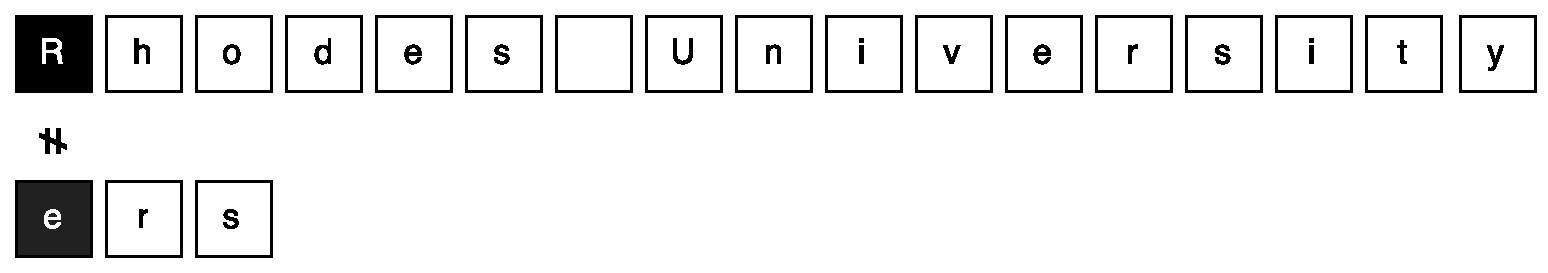
\includegraphics[width=\textwidth]{images/naive-1}
  \caption{The Na{\"i}ve algorithm compares the first letter of the search term to the first letter of the text.}
  \end{subfigure}
  
  \begin{subfigure}{\textwidth}
  \makeatletter
  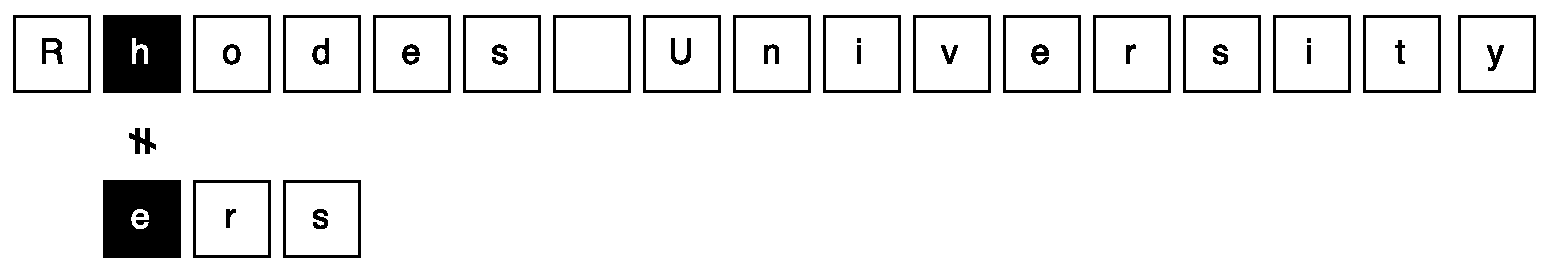
\includegraphics[width=\textwidth]{images/naive-2}
  \caption{Because the first letter of the search term did not match the first letter of the text, the Na{\"i}ve algorithm now compares the second letter of the text to the first letter of the search term.}
  \end{subfigure}
  
  \begin{subfigure}{\textwidth}
  \makeatletter
  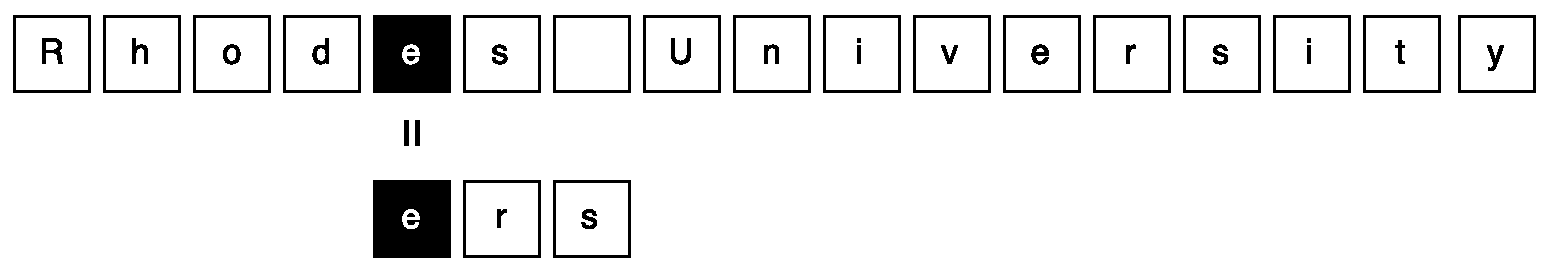
\includegraphics[width=\textwidth]{images/naive-3}
  \caption{After some iteration, the first letter of the search term is matched against the fifth letter of the text.}
  \end{subfigure}
  
  \begin{subfigure}{\textwidth}
  \makeatletter
  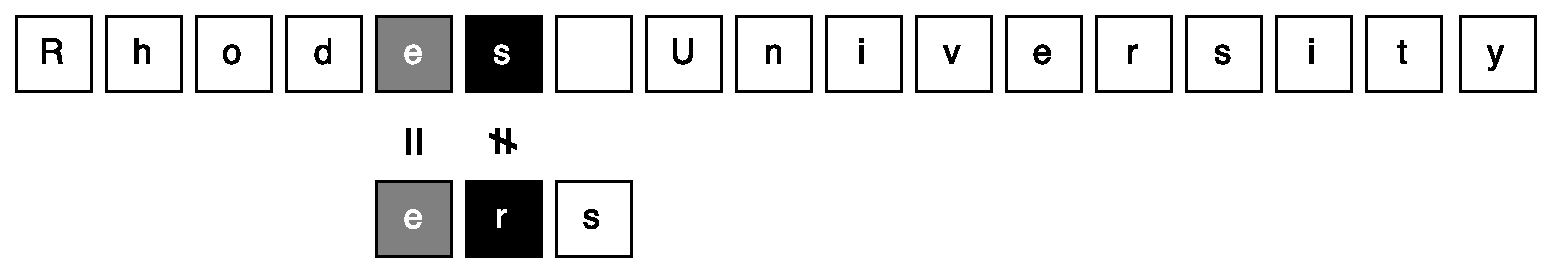
\includegraphics[width=\textwidth]{images/naive-4}
  \caption{The next letter of the text does not match the second letter of the search term. A match is not declared.}
  \end{subfigure}
  
  \begin{subfigure}{\textwidth}
  \makeatletter
  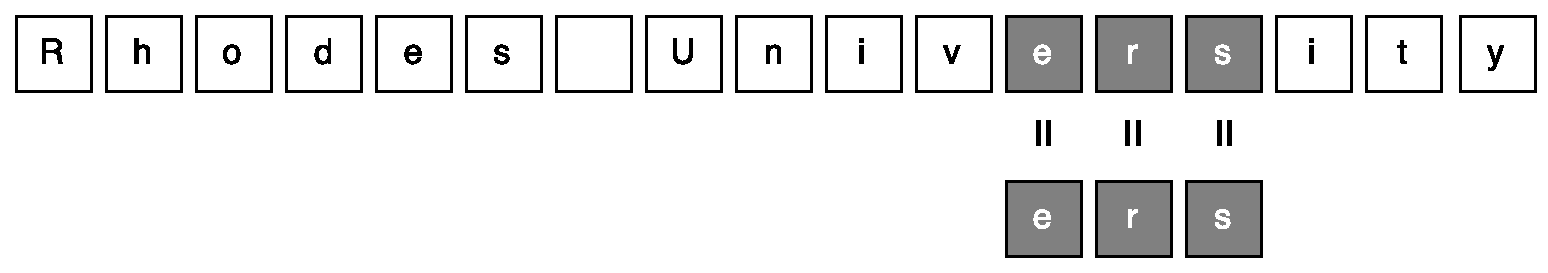
\includegraphics[width=\textwidth]{images/naive-5}
  \caption{As before letters from the search term match letters in the text. In this case the entirety of the search term was matched in the text and so a match is declared.}
  \end{subfigure}
  
  \caption{The process by which the Na{\"i}ve algorithm conducts its search}
  
\end{figure}

\subsection{Aho-Corasick}
This string search algorithm, originally proposed by \cite{Aho1975}, matches all search terms simultaneously.

The Aho-Corasick algorithm was designed as an improvement on the trie (or keyword tree). A trie works by constructing a tree where each edge is labeled by a character and each node is the concatenation of edges leading up to the node. Nodes are then labeled with the index of the corresponding search term. For the search terms: he, she, his, hers (\(P = \{he, she, his, hers\}\)); the following trie can be constructed: 

\begin{figure}[hbt]
  \label{trie}
  \centering
  \makeatletter
  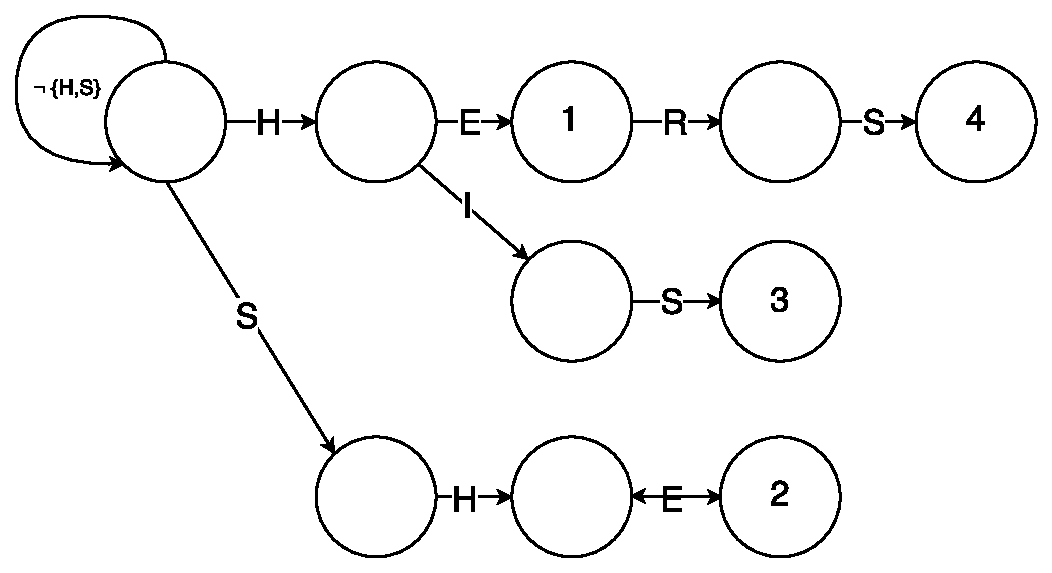
\includegraphics[width=\textwidth]{images/trie.pdf}
  \caption{Trie (keyword tree) for the search terms \(P = \{he, she, his, hers\}\)}
\end{figure}

A lookup through a trie done by starting at the root, follow a path by matching the packet data against the edge labels for as long as possible. If the path leads to a node that is labeled: the string is a search term. If the path terminates at a node that does not have a label then no match is made. Lookups have \(O(nm)\) time complexity.

As stated, the Aho-Corasick algorithm is an extension of the trie. The algorithm extends the trie into an automaton. The following functions are defined to determine the subsequent action given the current node and character being inspected: goto, failure and output.

\subsubsection{The goto function} \label{goto-function}

Defined as \(g(q, a)\), the goto function gives the next state by taking the current state (or node) \(q\) and a matching character \(a\) as parameters. If an edge \((q, v)\) has the label \(a\) then the goto function is defined as \(g(q, a) = v\). \(g(0, a) = 0\) for any \(a\) that does not have an edge labeled out of the root node. For anything else \(g(q, a) =  \emptyset\).

\subsubsection{The failure function} \label{failure-function}

The failure function, or \(f(q)\), defines the next state if no suitable state from the goto function has been found. In other words, when a mismatch occurs. The failure function finds the longest suffix of the label at \(q\) which is a prefix of a search term.

\subsubsection{The output function} \label{output-function}

The output function, \(out(q)\) defines all search terms that have been recognised when entering \(q\).

\begin{figure}[hbt]
  \label{trie}
  \centering
  \makeatletter
  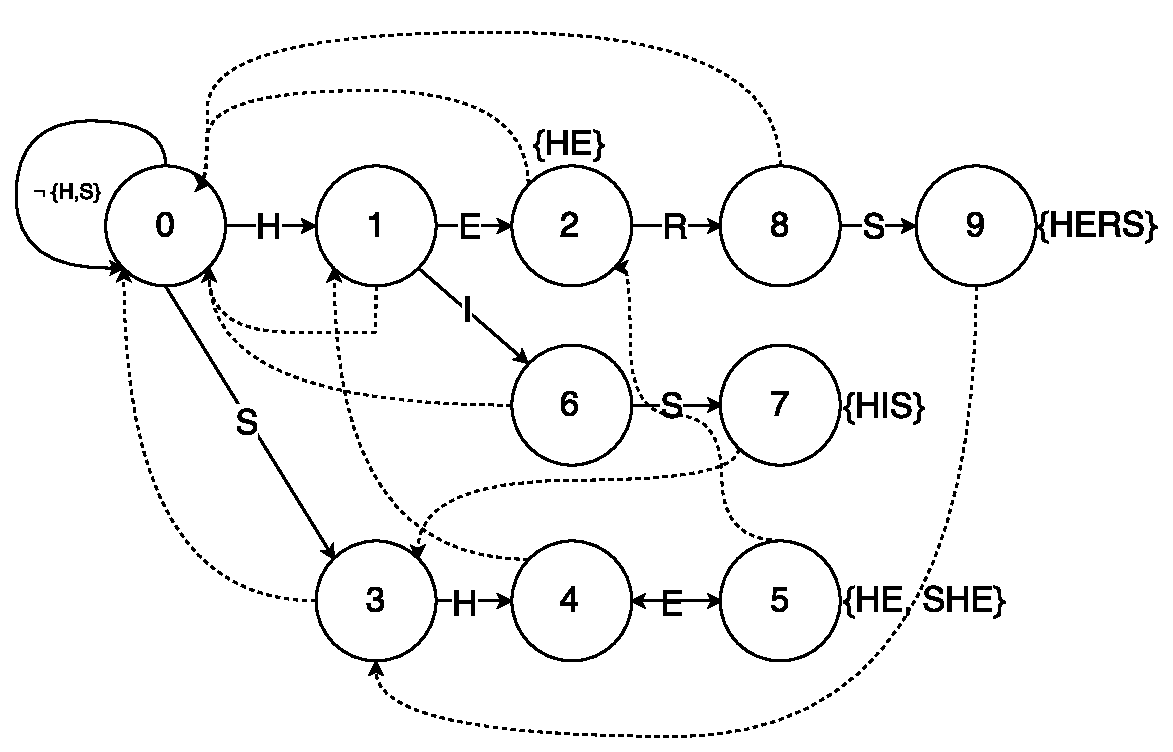
\includegraphics[width=\textwidth]{images/ac-automaton}
  \caption{Aho-Corasick Automaton for \(P = \{he, she, his, hers\}\)}
\end{figure}

The algorithm has a proven linear time complexity proportional to the sum of the length of the packet, the search terms and the number of times a term is matched \citep{Aho1975}. Formally it has O(\(n + m + z\)) where \(n\) is the length of the packet payload, \(m\) is the length of the search terms and \(z\) is the number of times the pattern is matched.

With the small initial overhead encountered when constructing the automaton (computing the goto [see \ref{goto-function}] , failure [see \ref{failure-function}] and output [see \ref{output-function}] functions), the Aho-Corasick algorithm can shave off precious time by eliminating unnecessary work using the failure functions.

\subsection{Bitap}

Best known for its use in agrep (reference?), the Bitap algorithm \cite{Baeza1992} is an approximate string matching algorithm. That is to say that for a given search term and substring of text, the Bitap algorithm can tell you if those elements are approximately equal. The algorithm's speed is due to its use of bitwise operations on precomputed bitmasks 

\subsection{Bloom}

A Bloom filter, first proposed by \cite{Bloom1970}, is a data-structure used to determine whether something is a member of a set. Traditionally Bloom filters and other hash table-based algorithms have been used in networking applications such as routing, shallow packet inspection and network monitoring \citep{Song2005}›. In the context of packet inspection a Bloom filter is used to see if a substring of the packet payload is a member of the set containing all search terms.

A bloom filter works by hashing each of the search terms a number of times, for each hash a bit is set in a corresponding bit vector. Lookup in a bloom filter involves hashing the string that you want to look up each time for each bit vector and checking to see if the bits are set. The price for efficient such efficient lookup is that a bloom filter can only tell you if a string in definitely not in the set. It can only say with a non-100 percent certainty if the string matches a search term.

\begin{figure}[hbt]
  \label{bloom-1}
  \centering
  
  \begin{subfigure}{\textwidth}
  \makeatletter
  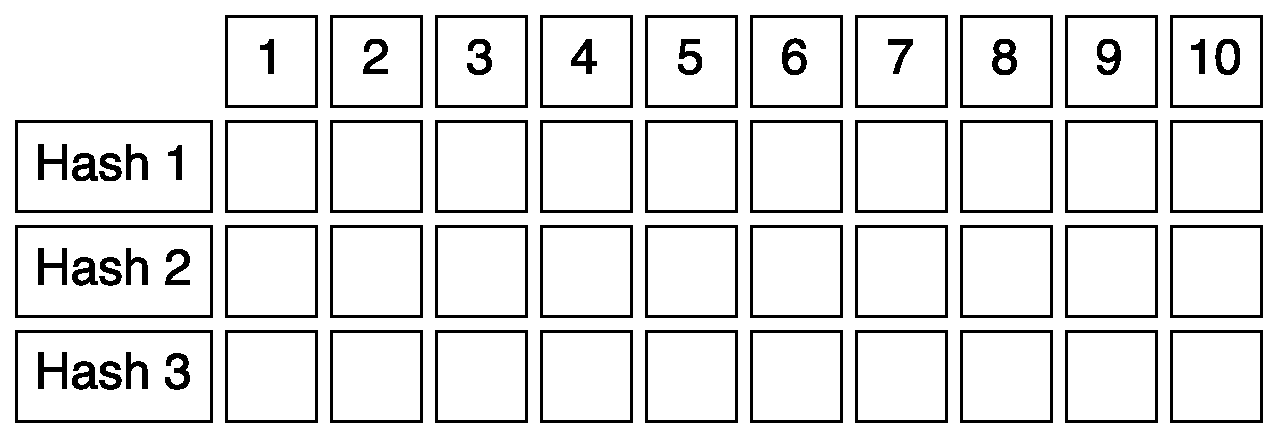
\includegraphics[width=\textwidth]{images/bloom-1}
  \caption{The bloom filter initially starts with hash tables initialised to zero, one for each of the hash functions being used.}
  \end{subfigure}
\end{figure} 

\begin{figure}[hbt]
  \ContinuedFloat  
  \label{bloom-2}
  \centering
  \begin{subfigure}{\textwidth}
  \makeatletter
  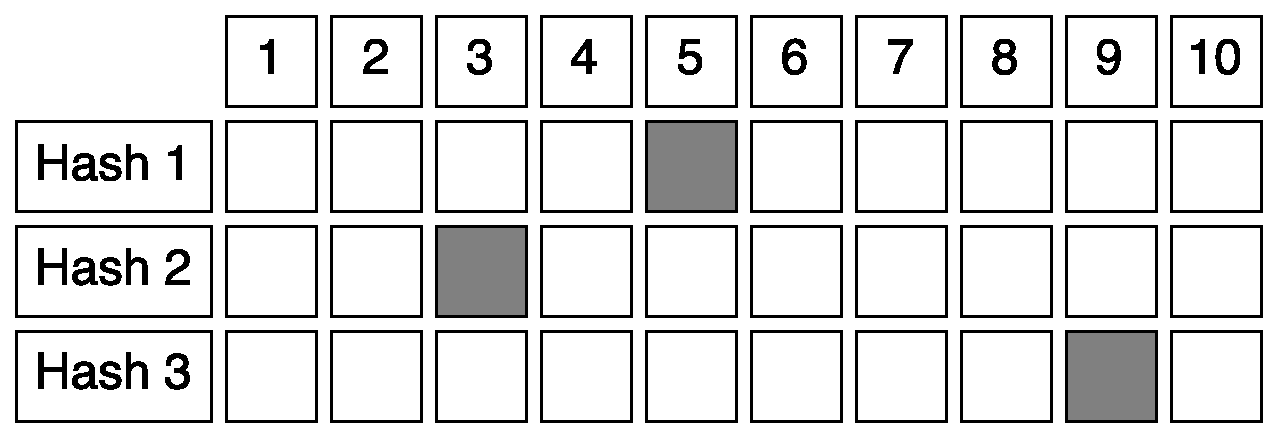
\includegraphics[width=\textwidth]{images/bloom-2}
  \caption{The first search term is hashed by each of the hashing algorithms, for each algorithm a single value is returned. The place in the hash table corresponding to the value is set. Here 5 is set for Hash 1, 3 for Hash 2 and 9 for Hash 10.}
  \end{subfigure}
\end{figure}

\begin{figure}[hbt]
  \ContinuedFloat  
  \label{bloom-3}
  \centering
  \begin{subfigure}{\textwidth}
  \makeatletter
  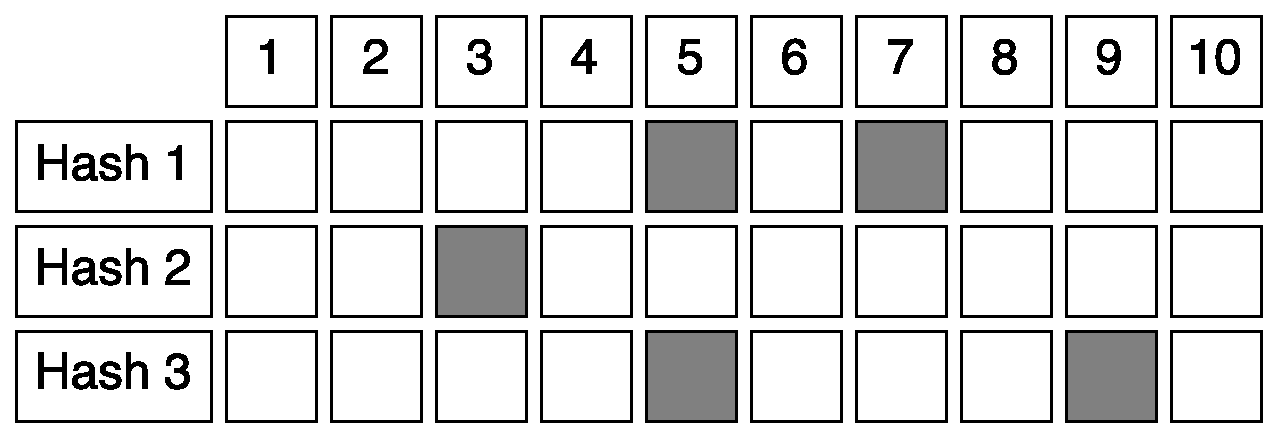
\includegraphics[width=\textwidth]{images/bloom-3}
  \caption{A second search term is put through the three hashing functions. For this term Hash 1 gives the value of 7, Hash 2 gives 3 and Hash 3 gives 5. Note that Hash 2 has given the same values for both search terms.}
  \end{subfigure}
\end{figure}

\begin{figure}[hbt]
  \ContinuedFloat  
  \label{bloom-4}
  \centering
  \begin{subfigure}{\textwidth}
  \makeatletter
  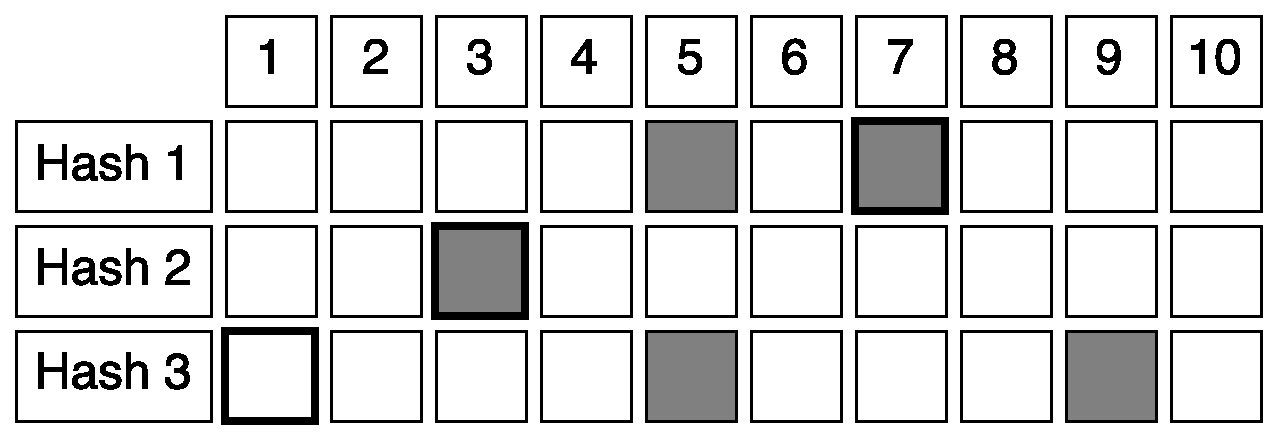
\includegraphics[width=\textwidth]{images/bloom-4}
  \caption{When doing a lookup in a Bloom table, a similar approach is used to insertion. The term being looked up is hashed by the various hashing algorithms and the hash tables are check to see if the corresponding bits are set. Here the first two hash tables show that the bits are set but the last hash table does not find a match. No match is declared.}
  \end{subfigure}
\end{figure}

\begin{figure}[hbt]
  \ContinuedFloat  
  \label{bloom-5}
  \centering
  \begin{subfigure}{\textwidth}
  \makeatletter
  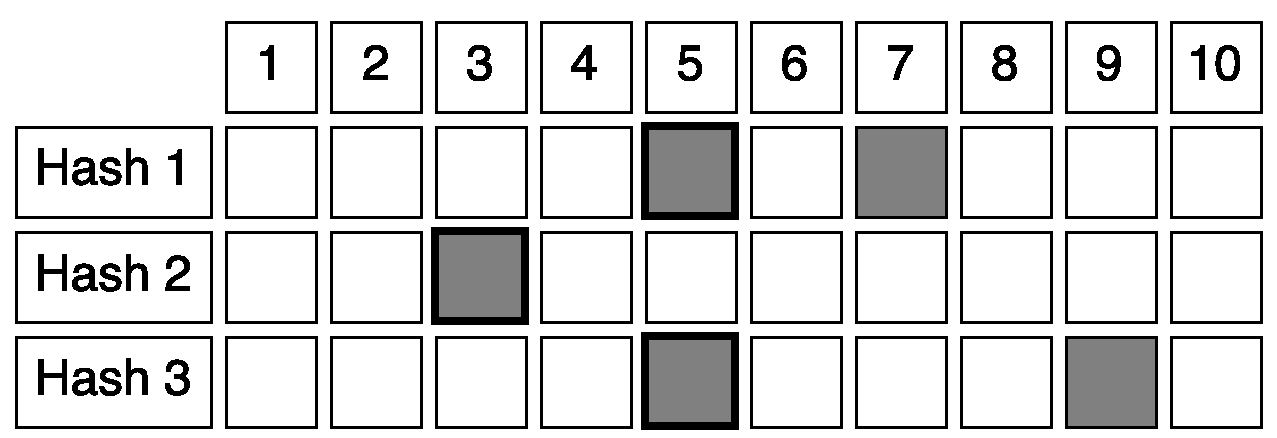
\includegraphics[width=\textwidth]{images/bloom-5}
  \caption{Another being of text is being evaluated. Here the text is put through the same three hashing algorithms and for each one a corresponding entry in the hash table is found. The Bloom filter declares this a likely match. The careful reader may notice that this is, in fact, not a match. Figures \ref{bloom-2} and \ref{bloom-3} show each term being added to the Bloom filter and the results of this search do not match the insertions.}
  \end{subfigure}
\end{figure}

\begin{figure}[hbt]
  \ContinuedFloat  
  \label{bloom-6}
  \centering
  \begin{subfigure}{\textwidth}
  \makeatletter
  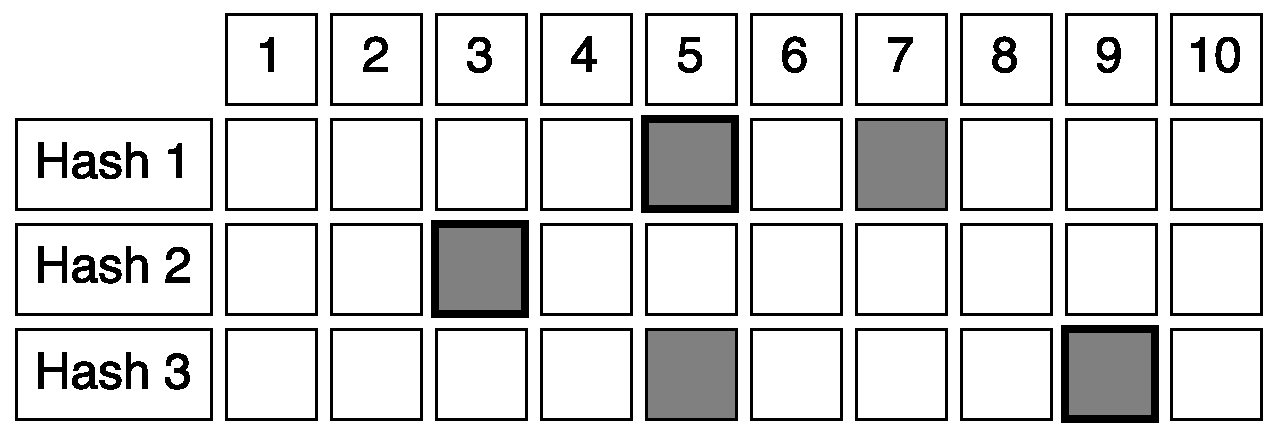
\includegraphics[width=\textwidth]{images/bloom-6}
  \caption{Another piece of text is put through the bloom filter with matches again appearing. These matches are not false positives as they correspond to the initially placed bit during the insertion phase.}
  \end{subfigure}
  \caption{The process of inserting into and doing a lookup on a Bloom filter.}
\end{figure}

\subsection{Boyer-Moore}

The Boyer-Moore algorithm \citep{Boyer1977} is an improved version of the Na{\"i}ve algorithm. It too uses a sliding window to compare the search string with substrings in the search text. Boyer-Moore's improvement on the Na{\"i}ve algorithm involves a pre-processing step whereby the algorithm determines certain ways that it can jump over text.

In the Na{\"i}ve algorithm, if during the matching of a word it fails halfway through, the algorithm simply starts at the next character. The Boyer-Moore uses its pre-processing step to determine if and how far along in the text the algorithm can jump. Thus making fewer comparisons and increasing the overall speed.

The Boyer-Moore algorithm works by comparing text from the rear to the front of the search pattern. If the character in the text does not match any character in the search pattern then the pattern can jump the length of the pattern forward. If the character is found somewhere within the search string then the pattern is shifted to where the characters line up and the process is then repeated.

\subsection{Cuckoo}
\cite{Fan2014}
\subsection{Horspool}
\cite{Horspool1980}
\subsection{Rabin-Karp}
\cite{Karp1987}
\subsection{Knuth-Morris-Pratt}
\cite{Knuth1977}

\section{Testing Environment}	
Give a run-down of the system used.

The Rust language was used to implement all of the search algorithms. Rust was selected because it is fast and safe. Both  qualities are important in a real-time packet inspection scenarios. For interacting with both packet captures and live capture handles we used the Rust pcap\footnote{\url{https://github.com/ebfull/pcap}} library. This library provides a wrapper around libpcap\footnote{\url{http://www.tcpdump.org/}}. Through pcap, we are able to easily retrieve the packet data which can in turn be run through the various algorithms (See part \ref{algorithms}).

Each algorithm was implemented in Rust. All but the Bloom\footnote{\url{https://github.com/nicklan/bloom-rs}} \cite{Bloom1970} and Cuckoo\footnote{\url{https://github.com/seiflotfy/rust-cuckoofilter}} \cite{Fan2014} filters were were implemented by the authors.

Talk about the pcap format.

The data used in the tests was real-world packet data collected the DNS servers of local schools. The libpcap library, in conjunction with tcpdump was used to collect and save the packet information. The total number of captured packets was culled to a reasonable one million packets to allow for reasonable processing and interpretation times.

Each algorithm was separately run over the dataset for a variety of search terms.

Search terms: google, amazonaws.com

Books: Alices-Adventures-in-Wonderland.txt, Pride-and-Prejudice.txt, The-Prince.txt, Bird-Watching.txt, The-Adventures-of-Sherlock-Holmes.txt, The-Yellow-Wallpaper.txt, Frankenstein-or-the-Modern-Prometheus.txt, and The-Adventures-of-Tom-Sawyer-Complete.txt.

\begin{comment}
 To get the size of each file:
    $ find . -name '*.cap' | xargs du -h
 To get the number of packets in each file:
    $ find . -name '*.pcap' | xargs wc
 The previous one may be incorrect.
\end{comment}

\section{Results}
Have some tables of general speeds across the various algorithms/datasets. Same for memory.

\section{Analysis}
Compare results with each other.

Compare results against the theoretical outcomes.

\section{Conclusion}
Talk about going forward. Future work.
\nocite{*}


\bibliographystyle{apalike}
\bibliography{bibliography}

\end{document}